\section{RISC-V ISA and Extensions}

The RISC-V instruction set architecture (ISA) is an open and modular standard that provides a simplified, extensible foundation for a wide range of computing applications. Its modularity is one of its most significant features, allowing users to start with a small set of base instructions and then tailor the ISA with custom extensions, making it particularly suitable for specialized domains such as edge computing and artificial intelligence.

At its core, the RISC-V base ISA includes only the essential integer arithmetic instructions, such as load/store, branch, and basic arithmetic operations. These instructions form the basis of the RV32I subset, which operates on 32-bit data and provides all the necessary functionalities to execute fundamental computing tasks. The RV32I set consists of 47 instructions encoded in a fixed 32-bit format, with fields specifying operation types, operand registers, and immediate values, as shown in Fig.~\ref{fig:riscvisa}. The opcode is a key part of this encoding, determining the nature of the operation, while other fields like funct3 and funct7 define more specific operations or variations of the base instruction.

\begin{figure}
    \centering
    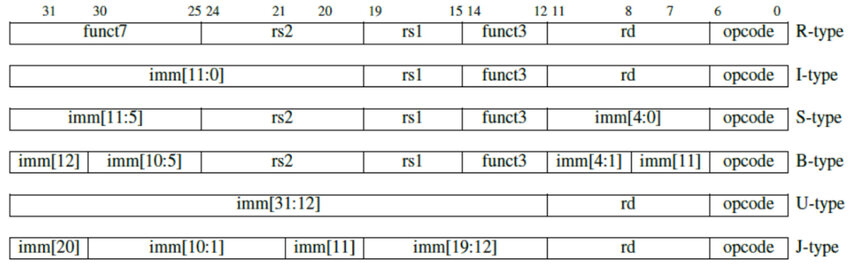
\includegraphics[width=0.8\textwidth]{figures/riscvisa.png}
    \caption{RISC-V 32-bit instruction encoding format \cite{RISCVISA}}
    \label{fig:riscvisa}
\end{figure}

The 32-bit encoding format allows for compact and efficient instruction decoding and execution, which is one of the key advantages of RISC-V in embedded systems and low-power applications. Each instruction is defined by specific bit fields: \cite{RISCVISA}
\begin{itemize}
    \item \textbf{Opcode}: Specifies the instruction type, such as arithmetic, memory access, or control flow.
    \item \textbf{rd}: Destination register for the result.
    \item \textbf{funct3}: Further categorizes the instruction within the opcode type.
    \item \textbf{rs1} and \textbf{rs2}: Source registers.
    \item \textbf{funct7}: Provides additional specificity for certain operations, such as shifts and bitwise operations.
\end{itemize}

RISC-V's open standard encourages customization, and one of its most powerful features is the ability to add custom instructions to enhance performance for domain-specific tasks. These custom instructions are often introduced as extensions to the RV32I base. A popular extension is the addition of SIMD (Single Instruction, Multiple Data) instructions, enabling parallel data processing.

To implement custom operations as an extension to RV32I, one must define new opcodes or use available encoding spaces within the existing format. Custom instructions can be integrated into the existing pipeline, and tools like assembler and compiler must be modified to recognize these new instructions. In this thesis, custom instructions are designed to evaluate the benchmarks in MLonMCU framework. By targeting key operations in MLonMCU models, the custom instructions allow for more efficient processing of tasks, leading to significant improvements in performance.

In summary, the RISC-V ISA provides a robust and flexible foundation with RV32I being its base subset. By utilizing its open and modular nature, this work extends the architecture with custom instructions tailored for MLonMCU model acceleration, showcasing the true potential of RISC-V for domain-specific optimization.

\section{LLVM}

LLVM (Low-Level Virtual Machine) is a versatile compiler infrastructure that supports the compilation of various programming languages to multiple target architectures. Its architecture consists of a collection of reusable compiler and toolchain technologies, providing a robust framework for both frontend and backend development.

At its core, LLVM employs an intermediate representation (IR) that serves as a common code representation between source languages and target architectures. This IR is designed to be language-agnostic and can be optimized independently of the source code, enabling a wide range of optimization techniques to be applied uniformly across different languages.

One of the key features of LLVM is its modularity, which allows developers to extend the compiler with new optimizations or target architectures without modifying existing components. This flexibility is particularly advantageous for research and development in custom instruction sets, facilitating rapid prototyping and experimentation.

\begin{figure}
    \centering
    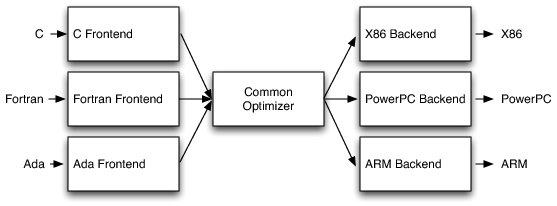
\includegraphics[width=0.8\textwidth]{figures/llvm.png}
    \caption{LLVM compilation process. \cite{llvmfigure}}
    \label{fig:llvm}
\end{figure}

The compilation process in LLVM (See Fig.~\ref{fig:llvm}) typically comprises several stages:

\begin{enumerate}
    \item \textbf{Frontend:} This component parses the source code and converts it into LLVM IR. Frontends can be developed for various programming languages, allowing LLVM to serve as a backend for diverse ecosystems.

    \item \textbf{Optimization:} Once in IR form, LLVM applies a series of optimization passes that enhance performance, reduce code size, and improve overall efficiency. These optimizations can be tailored based on the specific characteristics of the target architecture.

    \item \textbf{Backend:} The backend is responsible for generating machine code specific to the target architecture. It leverages target-specific information to produce optimized and efficient binaries.
\end{enumerate}

In the context of custom instruction sets, LLVM's design allows for seamless integration of vendor-defined extensions. By defining new instruction patterns and leveraging existing optimization frameworks, developers can enhance the performance of their applications without requiring deep knowledge of the underlying compiler infrastructure \cite{llvm}.

Overall, LLVM provides a powerful platform for compiling and optimizing code, making it an ideal choice for implementing and exploring custom ISAs. The capabilities of LLVM, particularly its support for autovectorization and advanced optimization techniques, directly align with the objectives of this research, facilitating the effective utilization of custom instruction sets in performance-critical applications.


\section{M2-ISA-R}
M2-ISA-R is a framework designed to facilitate the description and implementation of custom ISAs. It uses a metamodel-based approach that allows for a high level of abstraction when specifying both functional and structural components of a processor architecture. This flexibility in modeling makes it particularly useful for hardware-software co-design.

\begin{figure}
    \centering
    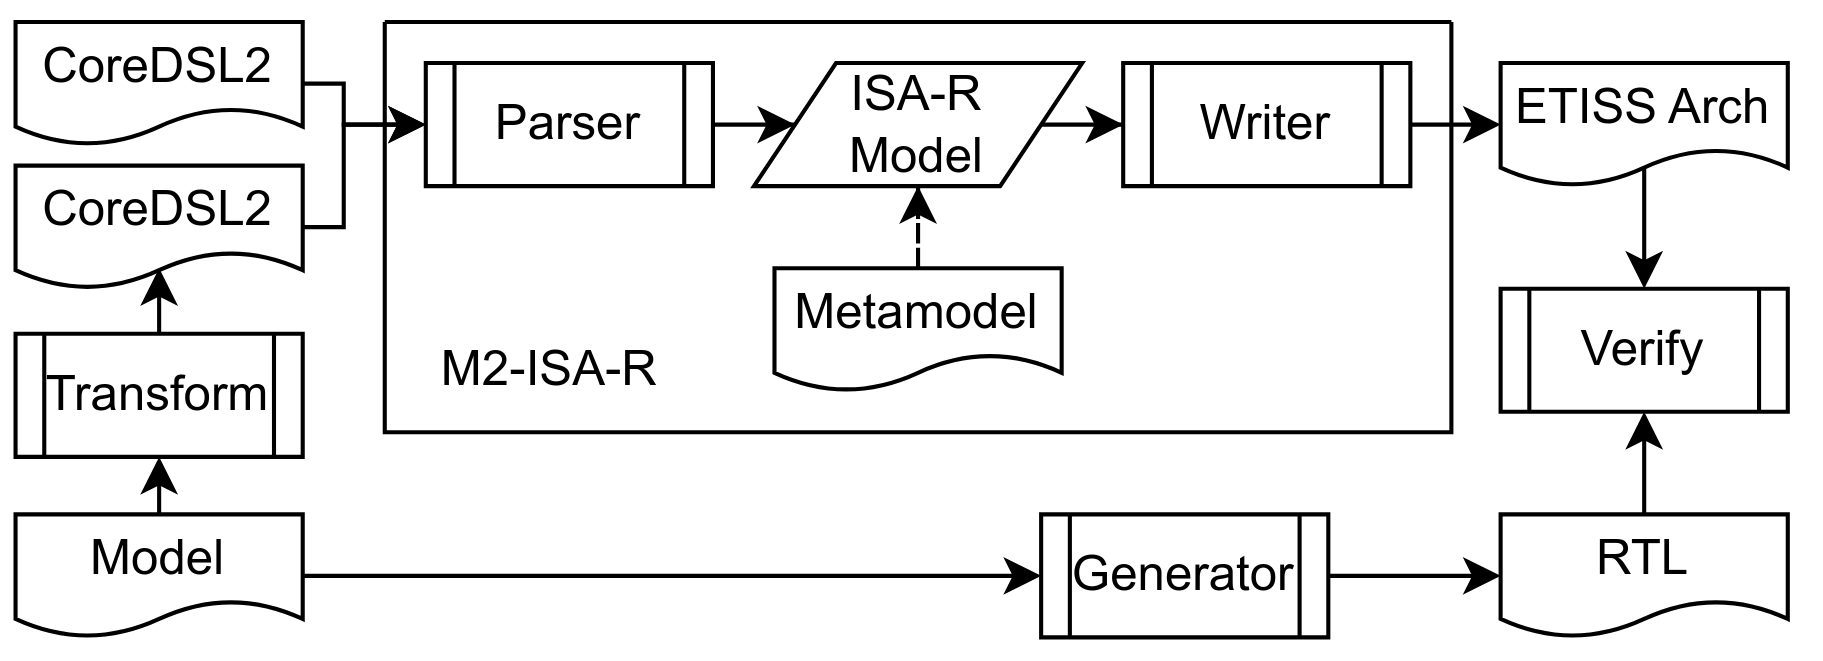
\includegraphics[width=0.8\textwidth]{figures/m2isar.png}
    \caption{M2-ISA-R workflow \cite{RISCVSimulation}}
    \label{fig:m2isar}
\end{figure}

The workflow (Fig.~\ref{fig:m2isar}) of M2-ISA-R involves parsing the ISA description via a frontend that utilizes the ANTLR4 framework. It then generates Python-based metamodel classes to capture both the architectural and behavioral aspects of the processor. The backend produces architecture-specific plugins for simulation tools, the most important of which is the ETISS architecture plugin. This enables rapid creation of CPU models for ETISS, closing the gap between high-level ISA descriptions and functional simulation.

In this research, M2-ISA-R has been employed to automatically generate the ETISS CPU architecture plugin for a custom ISA, allowing the seamless integration of this architecture into the ETISS simulation framework. This significantly reduces the development time needed for functional verification and performance simulation of custom CPU designs \cite{RISCVSimulation}.

\section{Seal5}

This work builds upon the Seal5 framework, which provides a semi-automated flow for generating LLVM compiler support for custom RISC-V instruction set architectures (ISAs). Seal5 leverages a C-style ISA description language to facilitate the integration of vendor-defined instructions, allowing for efficient exploration and implementation of custom instructions tailored to specific applications.

Seal5 enables the automatic generation of LLVM patches that cover a wide range of functionalities, from baseline assembly-level support to sophisticated compiler code generation patterns for scalar and vector instructions. The tool features a novel pattern generator approach focused on optimizing code generation for SIMD (Single Instruction, Multiple Data) instructions, including autovectorization capabilities.

By utilizing Seal5, this research aims to convert a custom instruction set into a customized LLVM backend. This process significantly reduces development time and effort while achieving performance levels comparable to or exceeding those of manually implemented LLVM toolchains. The ability of Seal5 to support autovectorization enhances the execution efficiency of workloads, making it an invaluable asset for the exploration of custom ISA extensions \cite{Seal5}.

\section{MLonMCU}
MLonMCU is a benchmarking tool designed specifically for TinyML applications, enabling extensive performance evaluations across various models, frameworks, and hardware platforms. It is a flexible, framework-independent solution that allows for rapid retargeting to different platforms and devices. MLonMCU supports multiple TinyML frameworks, including TensorFlow Lite for Microcontrollers (TFLM) and MicroTVM, among others, offering a unified interface to compare the performance of machine learning models on embedded devices.

Key design principles of MLonMCU include isolation, reproducibility, parallelism, and extensibility. The tool isolates dependencies across different environments, ensuring that benchmarking sessions are not affected by other processes running on the system. It allows users to access all intermediate artifacts generated during a benchmarking session, ensuring full reproducibility of results. Furthermore, MLonMCU makes use of all available computational resources to run benchmarks in parallel, significantly speeding up the evaluation process. It also provides an extensible API, allowing users to integrate custom components and features easily.

MLonMCU's workflow consists of several stages, including model loading, compilation, and execution on target devices or simulators. It also supports post-processing stages for result analysis, where it generates detailed reports on metrics such as execution latency, instructions per cycle, runtime, and memory usage. The platform-agnostic design of MLonMCU ensures that it can handle a wide variety of devices out of the box, making it an ideal tool for early-stage design evaluations and virtual prototyping.

In this research, MLonMCU is used to evaluate the performance of translated instruction sets across different machine learning models. The benchmarking results provide crucial insights into how well the custom instruction sets perform in terms of execution efficiency and resource usage across various target platforms \cite{MLonMCU}.